% move all configuration stuff into one file so we can focus on the content
\documentclass[aspectratio=169,hyperref={pdfpagelabels=false,colorlinks=true,linkcolor=white,urlcolor=blue},t]{beamer}

%%%%%%%%%%%%%%%%%%%%%%%%%%%%%%%%%%%%%%%%%%%%%%%%%%%%%%%%%%%%%%%%%%%%%%%%%%%%%%%%%%
%%%%%%%%%%%%%%%%%%%%%%%%%%%%%%%%%%%%%%%%%%%%%%%%%%%%%%%%%%%%%%%%%%%%%%%%%%%%%%%%%%
% packages
\usepackage{pict2e}
\usepackage{epic}
\usepackage{amsmath,amsfonts,amssymb}
\usepackage{units}
\usepackage{fancybox}
\usepackage[absolute,overlay]{textpos} 
\usepackage{media9} % avi2flv: "C:\Program Files\ffmpeg\bin\ffmpeg.exe" -i TuneFreqFilterbank.avi -b 600k -s 441x324 -r 15 -acodec copy TuneFreqFilterbank.flv
\usepackage{animate}
\usepackage{gensymb}
\usepackage{multirow}
\usepackage{silence}
\usepackage[backend=bibtex,style=ieee]{biblatex}
\AtEveryCitekey{\iffootnote{\tiny}{}}
\addbibresource{references}

%%%%%%%%%%%%%%%%%%%%%%%%%%%%%%%%%%%%%%%%%%%%%%%%%%%%%%%%%%%%%%%%%%%%%%%%%%%%%%%%%%
%%%%%%%%%%%%%%%%%%%%%%%%%%%%%%%%%%%%%%%%%%%%%%%%%%%%%%%%%%%%%%%%%%%%%%%%%%%%%%%%%%
% relative paths
\graphicspath{{graph/}}


%%%%%%%%%%%%%%%%%%%%%%%%%%%%%%%%%%%%%%%%%%%%%%%%%%%%%%%%%%%%%%%%%%%%%%%%%%%%%%%%%%
%%%%%%%%%%%%%%%%%%%%%%%%%%%%%%%%%%%%%%%%%%%%%%%%%%%%%%%%%%%%%%%%%%%%%%%%%%%%%%%%%%
% units
\setlength{\unitlength}{1mm}

%%%%%%%%%%%%%%%%%%%%%%%%%%%%%%%%%%%%%%%%%%%%%%%%%%%%%%%%%%%%%%%%%%%%%%%%%%%%%%%%%%
%%%%%%%%%%%%%%%%%%%%%%%%%%%%%%%%%%%%%%%%%%%%%%%%%%%%%%%%%%%%%%%%%%%%%%%%%%%%%%%%%%
% theme & layout
\usetheme{Frankfurt}
\beamertemplatenavigationsymbolsempty
%\setbeamertemplate{frametitle}[smoothbars theme]
\setbeamertemplate{frametitle}
{
    \begin{beamercolorbox}[ht=1.8em,wd=\paperwidth]{frametitle}
        \vspace{-.1em}%
        \hspace{.2em}{\strut\insertframetitle\strut}
        
        \hspace{.2em}\small\strut\insertframesubtitle\strut
        %\hfill
        %
\includegraphics[height=.8cm,keepaspectratio]{CenterMusicTechnology-solid-2lines-white-CoAtag}
        
    \end{beamercolorbox}
    \begin{textblock*}{100mm}(11.6cm,.7cm)
        \includegraphics[height=.8cm,keepaspectratio]{logo_GTCMT_black}
    \end{textblock*}
}

% set this to ensure bulletpoints without subsections
\usepackage{remreset}
\makeatletter
\@removefromreset{subsection}{section}
\makeatother
\setcounter{subsection}{1}

%---------------------------------------------------------------------------------
% appearance
\setbeamercolor{structure}{fg=gtgold}
\setbeamercovered{transparent} %invisible
\setbeamercolor{bibliography entry author}{fg=black}
\setbeamercolor*{bibliography entry title}{fg=black}
\setbeamercolor*{bibliography entry note}{fg=black}

%\usepackage{pgfpages}
%\setbeameroption{show notes}
%\setbeameroption{show notes on second screen=right}
%---------------------------------------------------------------------------------
% fontsize
\let\Tiny=\tiny

%%%%%%%%%%%%%%%%%%%%%%%%%%%%%%%%%%%%%%%%%%%%%%%%%%%%%%%%%%%%%%%%%%%%%%%%%%%%%%%%%%
%%%%%%%%%%%%%%%%%%%%%%%%%%%%%%%%%%%%%%%%%%%%%%%%%%%%%%%%%%%%%%%%%%%%%%%%%%%%%%%%%%
% warnings
\pdfsuppresswarningpagegroup=1
\WarningFilter{biblatex}{Patching footnotes failed}
\WarningFilter{latexfont}{Font shape}
\WarningFilter{latexfont}{Some font shapes}
\WarningFilter{gensymb}{Not defining}



\subtitle{Part 6.4: Polyphonic fundamental frequency detection}

%%%%%%%%%%%%%%%%%%%%%%%%%%%%%%%%%%%%%%%%%%%%%%%%%%%%%%%%%%%%%%%%%%%%%%%%%%%%
\begin{document}
    % generate title page
	

\begin{frame}
    \titlepage
    %\vspace{-5mm}
    \begin{flushright}
        \href{http://www.gtcmt.gatech.edu}{\includegraphics[height=.8cm,keepaspectratio]{logo_GTCMT_black}}
    \end{flushright}
\end{frame}


    \section[overview]{lecture overview}
        \begin{frame}{polyphonic pitch tracking}{overview}
            \begin{itemize}
                \item   \textbf{text book}  
                    \begin{itemize}
                        \item   \href{http://ieeexplore.ieee.org/xpl/articleDetails.jsp?tp=&arnumber=6331122&}{\underline{\textit{Chapter 5: Tonal Analysis} (pp.~103--106)}}
                    \end{itemize}
                \bigskip
                \item<2->   \textbf{lecture content}
                    \begin{itemize}
                        \item<2->   fundamental frequency detection in polyphonic signals
                            \begin{itemize}
                                \item   historic methods
                                \item   non-negative matrix factorization (NMF)
                                \item   other approaches
                            \end{itemize}
                    \end{itemize}
            \end{itemize}
        \end{frame}

    \section[intro]{introduction}
        \begin{frame}{polyphonic pitch tracking}{problem statement}
            \begin{itemize}
                \item monophonic detection:
                    \begin{itemize}
                        \item   exactly one fundamental frequency with sinusoidals at multiples of $f_0$ (harmonics)
                    \end{itemize}
                \item   polyphonic detection:
                    \begin{itemize}
                        \item   multiple/unknown number of fundamental frequencies with harmonics
                    \end{itemize}
            \end{itemize}
        \end{frame}
    \section[iterative subtraction]{iterative subtraction}
	\begin{frame}{polyphonic pitch tracking}{iterative subtraction: introduction}
        \begin{itemize}
            \item \textbf{principle}
                \begin{enumerate}
                    \item	find most salient fundamental frequency 
                        \begin{itemize}
                            \item   e.g., with monophonic pitch tracking
                        \end{itemize}
                    \item<2->	remove this frequency and related frequency components from signal
                        \begin{itemize}
                            \item   e.g., with subtraction
                        \end{itemize}
                    \item<3->	repeat until termination criterion
                        \begin{itemize}
                            \item   e.g., number of voices
                        \end{itemize}
                \end{enumerate}
            \bigskip
            \item<4->   \textbf{challenges}            
            \begin{itemize}
                \item<4->	reliably \textit{identify fundamental frequency} in a mixture
                \item<5->	\textit{identify/group components} and amount to subtract
                    \begin{itemize}
                        \item   overlapping components
                        \item   spectral leakage
                    \end{itemize}
                \item<6->	define \textit{termination criterion}
                    \begin{itemize}
                        \item   unknown number of voices
                        \item   overall energy
                        \item   \dots
                    \end{itemize}
            \end{itemize}
        \end{itemize}
	\end{frame}
	
	\begin{frame}{polyphonic pitch tracking}{iterative subtraction: Cheveign\'e}
		\begin{enumerate}
			\item	compute squared AMDF
				\begin{equation*}
					\mathrm{ASMDF}_{xx}(\eta,n) = \frac{1}{i_{\mathrm{e}}(n)-i_{\mathrm{s}}(n)+1}\sum\limits_{i=i_{\mathrm{s}}(n)}^{i_{\mathrm{e}}(n)}{\big(x(i)- x(i+\eta)\big)^2}
				\end{equation*}
			\item<2->	find fundamental frequency
				\begin{equation*}
					\eta_{\mathrm{min}} = \argmin \big(\mathrm{ASMDF}_{xx}(\eta,n)\big)
				\end{equation*}
			\item<3->	apply comb cancellation filter, IR:
				\begin{equation*}
					h(i) = \delta(i) - \delta(i-\eta_{\mathrm{min}})
				\end{equation*}
			\item<4->	repeat process
		\end{enumerate}			
	\end{frame}
	
	\begin{frame}{polyphonic pitch tracking}{iterative subtraction: Meddis}
		\begin{enumerate}
			\item	auditory pitch tracking:
				\begin{equation*}
					r_{zz} (c,n,\eta) = \sum\limits_{\eta = 0}^{\mathcal{K}-1}{z_c(i)\cdot z_c(i+\eta)}
				\end{equation*}
			\pause
			\item	detect most likely frequency for all bands
			\pause
			\item	remove all bands with a max at detected frequency
			\pause
			\item	reiterate until most bands have eliminated			
		\end{enumerate}
	\end{frame}
	
	\begin{frame}{polyphonic pitch tracking}{iterative subtraction: spectral}
		\begin{enumerate}
			\item	find salient fundamental frequency (e.g.\ auditory approach, HPS)
			\pause
			\item	estimate current model for harmonic magnitudes
			\pause
			\item	subtract the model spectrum
			\pause
			\item	repeat process
		\end{enumerate}
	\end{frame}
	
	\begin{frame}{polyphonic pitch tracking}{exhaustive search}
		\begin{enumerate}
			\item	define set of all possible fundamental frequencies
			\pause
			\item	compute all possible pairs of fundamental frequency
			\pause
			\item 	repeatedly filter the signal with two comb cancellation filters (all combinations)
			\pause
			\item	find combination with minimal output energy
		\end{enumerate}
	\end{frame}
	
	\begin{frame}{polyphonic pitch tracking}{Karjalainen and Tolonen 1/3}
		\begin{enumerate}
			\item	pre-whitening by frequency warped linear prediction
			\pause
			\item	filter bank: low-pass and high-pass band (cut-off: \unit[1]{kHz})
			\pause
			\item 	HWR and smoothing
			\pause
			\item	generalized ACF ($\beta = 2/3$):
						\begin{equation*}
							r_{xx}^\beta (\eta,n) = \mathfrak{F}^{-1}\left\{|X(\jom)|^\beta\right\} 
						\end{equation*}
		\end{enumerate}
	\end{frame}
	
	\begin{frame}{polyphonic pitch tracking}{Karjalainen and Tolonen 2/3}
		\begin{enumerate}
			\item	summary ACF
			\pause
			\item	harmonic ACF processing:
				\begin{enumerate}
					\item	define temporary function:
						\begin{equation*}
							r'(\eta) = HWR(r_{xx}^\beta (\eta,n)) 
						\end{equation*}
					\pause
					\item	resample:
						\begin{equation*}
							\eta' = \frac{\eta}{m}
						\end{equation*}
					\pause
					\item	compute linear interpolation
						\begin{equation*}
							r'_m(\eta) = r'(\eta) + \frac{\eta-m\eta'}{m}\big(r'(\eta'+1) - r'(\eta')\big)
						\end{equation*}
					\pause
					\item	update $r(\eta)$
						\begin{equation*}
							r'(\eta) = HWR\big(r'(\eta) - HWR(r'_m(\eta))\big) 
						\end{equation*}
				\end{enumerate}
		\end{enumerate}
	\end{frame}
	
	\begin{frame}{polyphonic pitch tracking}{Karjalainen and Tolonen 3/3}
        \figwithmatlab{Karjalainen}
	\end{frame}
	
	\begin{frame}{polyphonic pitch tracking}{klapuri}
        %\vspace{-5mm}
        \begin{columns}[T]
            \column{.5\textwidth}
                \begin{enumerate}
                    \item	gammatone \textbf{filterbank} (100 bands)
                    \item<2->	\textbf{normalization}, HWR, smoothing, \ldots
                    \item<3->	\textbf{STFT} per filter channel (magnitude)
                    \item<4->	use \textbf{delta pulse templates} to detect frequency patterns
                    \item<5->	\textbf{pick most salient frequencies}, remove them
                \end{enumerate}
            \column{.5\textwidth}
                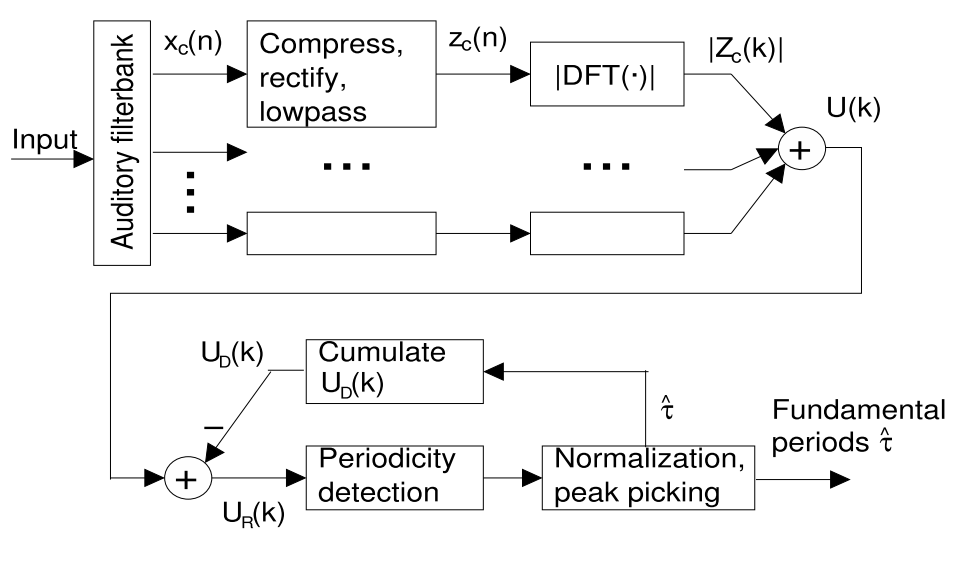
\includegraphics[scale=.25]{pitch_klapuri}
        \end{columns}
    \bigskip
    
    \begin{flushright}
        graph from \footfullcite{klapuri_perceptually_2005}
    \end{flushright}
	\end{frame}
    
	\begin{frame}{polyphonic pitch tracking}{NMF}
	\end{frame}
	\begin{frame}{polyphonic pitch tracking}{statistical approaches}
	\end{frame}
            
   \section[summary]{lecture summary}
        \begin{frame}{summary}{lecture content}
            \begin{enumerate}
                \item    name three basic approaches to detect the fundamental frequency (monophonic) and discuss strengths and weaknesses
                \smallskip
                \item<2->  what are the typical challenges for polyphonic pitch trackers?
                \smallskip
                \item<3->    what are potential problems when using NMF for pitch detection
            \end{enumerate}
        \end{frame}
\end{document}

